\title{ A Traveling Salesman Solution For The Capitals of All African Nations }
\author{
        Brian Gianforcaro \\
                Department of Computer Science\\
        Rochester Institute of Technology\\
}

\date{\today}

\documentclass[12pt]{article}

\usepackage{graphicx}
\usepackage{multicol}
\usepackage{mdwlist}

\begin{document}
\maketitle

\begin{abstract}
A Traveling Salesman Problem is the task of finding 
the shortest round trip path a traveling salesperson can take 
to visit each vertex of a given graph.  They are usually 
implemented using a genetic algorithm. Our salesperson
happens to be traveling to the capitals of every country in Africa that is a recognized member of the United Nations.
\end{abstract}

\section{The Problem}

\begin{figure}
\begin{center}
\setlength\fboxsep{1.00pt}
\setlength\fboxrule{1.00pt}
\fbox{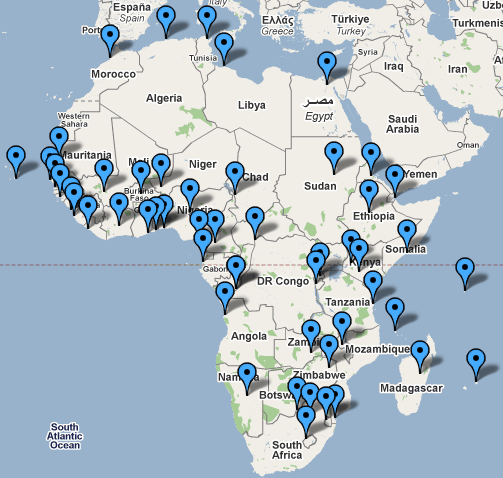
\includegraphics[scale=0.80]{points.png}}
\caption{Capitals of African Nations}
\end{center}
\end{figure}


\begin{multicols}{3}
\tiny\begin{enumerate*}
\item Algeria - Algiers
\item Angola - Luanda
\item Benin - Porto-Novo
\item Botswana - Gaborone
\item Burkina Faso - Ouagadougou
\item Burundi - Bujumbura
\item Cameroon - Yaounde
\item Cape Verde - Praia
\item Central African Republic - Bangui
\item Chad - N'Djamena
\item Comoros - Moroni
\item Congo, Republic of the - Brazzaville
\item Congo, Democratic Republic of the - Kinshasa
\item Cote d'Ivoire - Yamoussoukro
\item Djibouti - Djibouti
\item Egypt - Cairo
\item Equatorial Guinea - Malabo
\item Eritrea - Asmara
\item Ethiopia - Addis Ababa
\item Gabon - Libreville
\item The Gambia - Banjul
\item Ghana - Accra
\item Guinea - Conakry
\item Guinea-Bissau - Bissau
\item Kenya - Nairobi
\item Lesotho - Maseru
\item Liberia - Monrovia
\item Libya - Tripoli
\item Madagascar - Antananarivo
\item Malawi - Lilongwe
\item Mali - Bamako
\item Mauritania - Nouakchott
\item Mauritius - Port Louis
\item Morocco - Rabat
\item Mozambique - Maputo
\item Namibia - Windhoek
\item Niger - Niamey
\item Nigeria - Abuja
\item Rwanda - Kigali
\item Senegal - Dakar
\item Seychelles - Victoria
\item Sierra Leone - Freetown
\item Somalia - Mogadishu
\item South Africa - Pretoria 
\item Sudan - Khartoum
\item Swaziland - Mbabane
\item Tanzania - Dar es Salaam
\item Togo - Lome
\item Tunisia - Tunis
\item Uganda - Kampala
\item Zambia - Lusaka
\item Zimbabwe - Harare
\end{enumerate*}
\end{multicols}

\section{Overview}
The remainder of this article is organized as follows.
Section~ gives account of previous work.
Our new and exciting results are described in Section~.
Finally, Section gives the conclusions.

\section{Programs}

The TSP was solved using the Python 2.6 programming language.

I leveraged software written by John Montgomery 

The results were then visualized using Google maps mapping API. 

Two methods were 

\section{Solution}

\begin{figure}
\begin{center}
\setlength\fboxsep{1.00pt}
\setlength\fboxrule{1.00pt}
\fbox{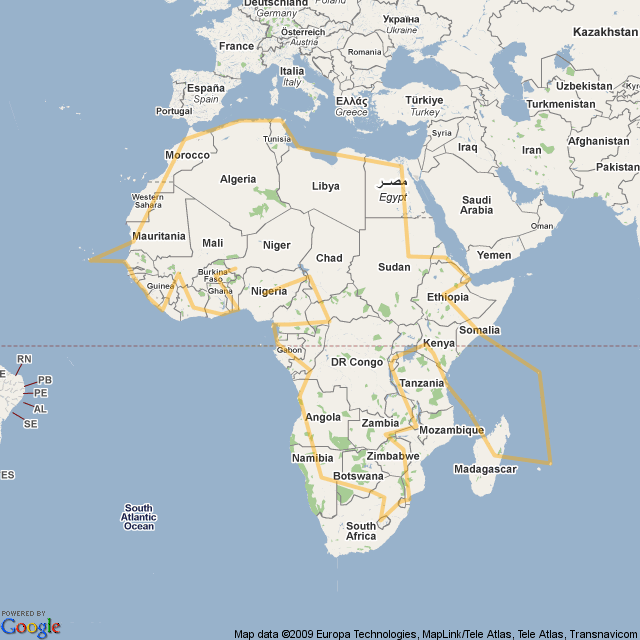
\includegraphics[scale=0.65]{path.png}}
\caption{Final Path Through Africa}
\end{center}
\end{figure}

In this section we describe the results.

\section{Runtime}
We worked hard, and achieved very little.

\section{Analysis}

\end{document}
